\question From the following: pick one to solve. If you solve more than one, you will receive credit for the problem with the highest score.

\begin{parts}
	\part A charge-neutral sphere of radius $R=0.05$ cm is situated in between the plates of a parallel plate capacitor with charge $Q=9$ nC. The top plate carries the negative charge (see the figure). What is the total electric flux through the sphere?
	
	\begin{figure}[ht!]
		\centering
		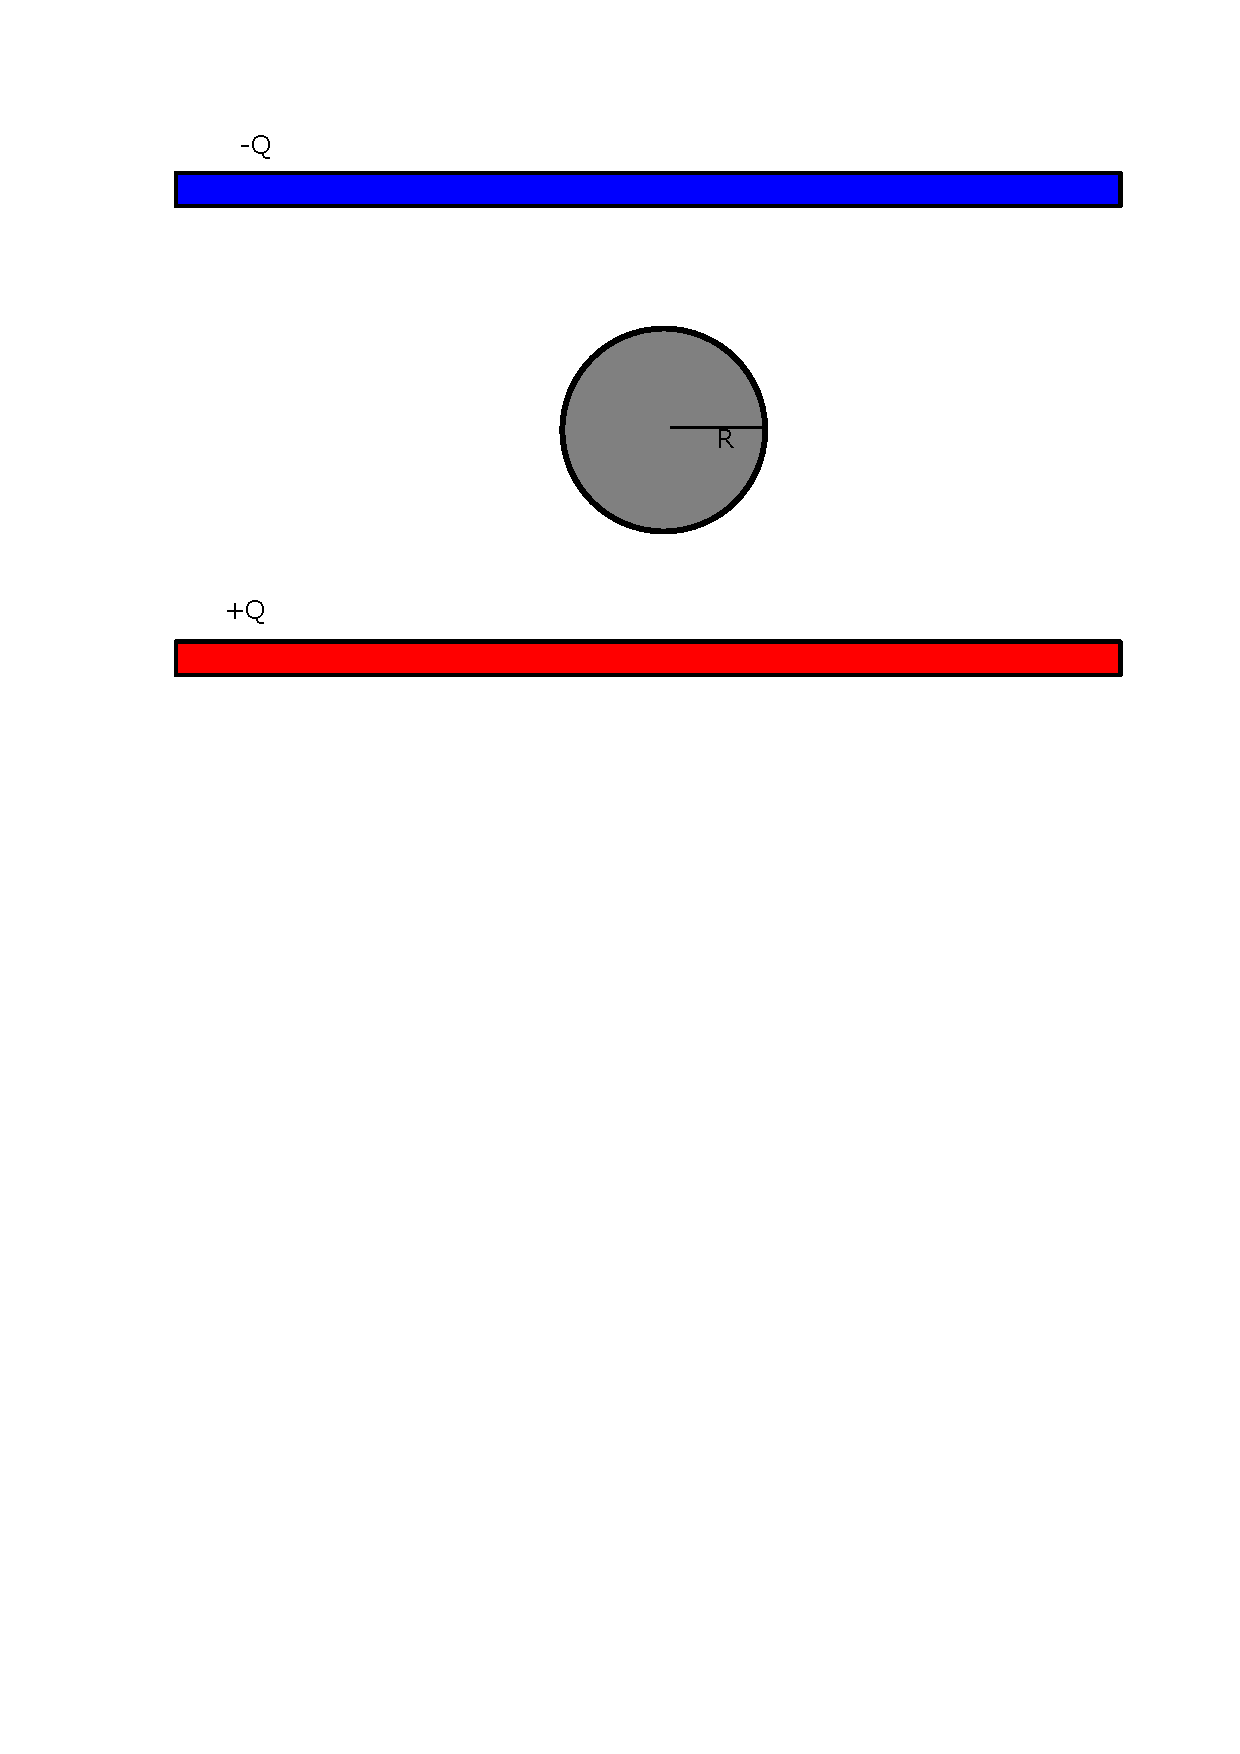
\includegraphics[width=8cm]{gauss.pdf}
	\end{figure}

\newpage

\part An electron (mass = 9.11$\times 10^{-31}$ kg) is released from rest a distance $d=12$ cm from the surface of a uniformly charged sphere with radius $R=5$ cm and total charge $Q=12$ nC. What is the velocity of the electron immediately before it collides with the surface of the sphere?

\begin{figure}[ht!]
	\centering
	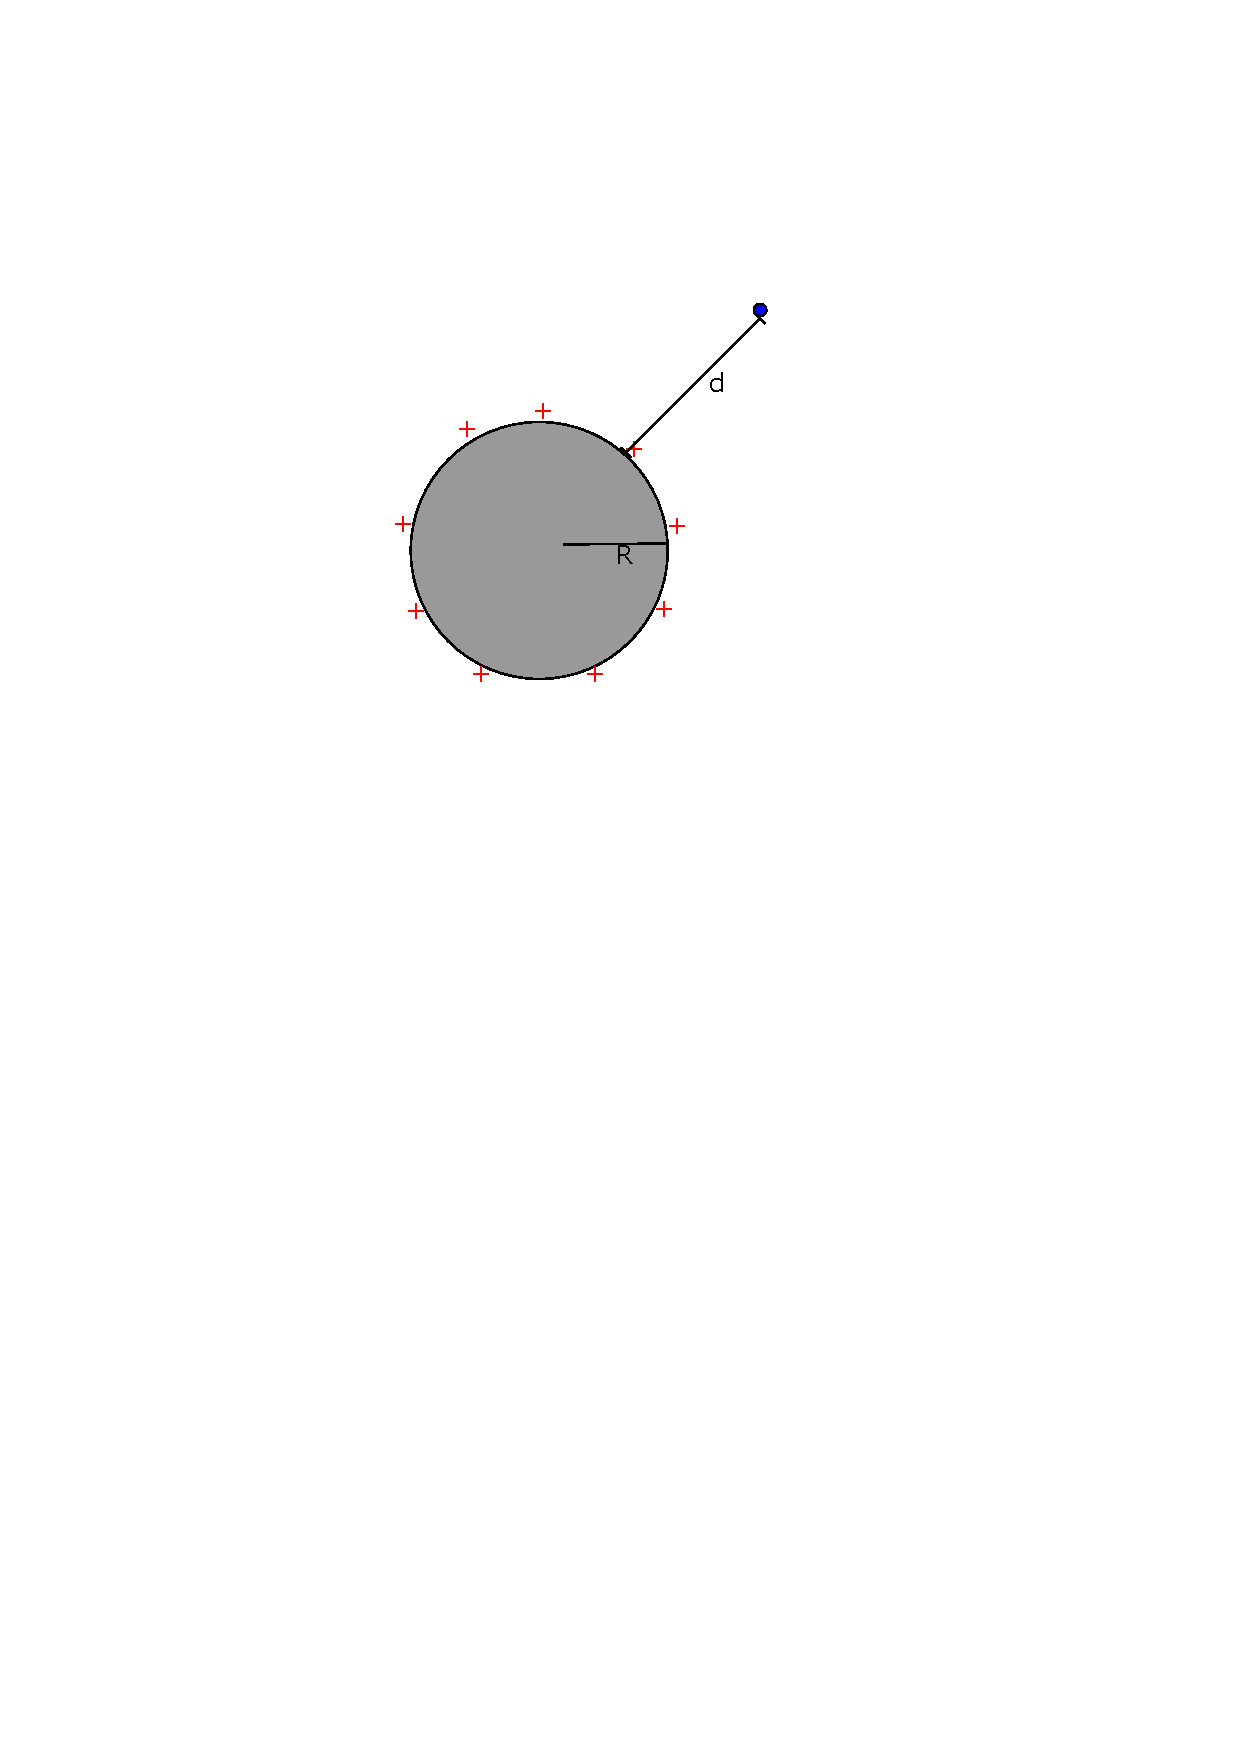
\includegraphics[width=5cm]{epotential.pdf}
\end{figure}
\end{parts}

